\section{Data}
\label{sec:data}

Three datasets are used throughout this work: the extended LoTSS-DR2 source sample, external morphology catalogues, and selected radio-relic cutouts. This chapter describes their selection and preparation, distinguishing the images used for model training and catalogue inference from the reference data used for comparison and the diffuse-emission application.

\subsection{LoTSS-DR2 sample selection and preprocessing}
\label{sec:data_catalogue}

The main catalogue dataset consists of the two LoTSS-DR2 products introduced in Sec.~\ref{sec:bg_lotss}:
\begin{itemize}
\item the \(6''\)-resolution Stokes~I mosaics provide the image data, with their \(1.5''\) pixel sampling used to construct the cutouts \citep{Shimwell2022}; and
\item the value-added catalogue of \citet{Hardcastle2023} supplies the source identifier, resolved-source flag, optical or infrared host coordinates, largest angular size (LAS), peak flux density, and mosaic identifier.
\end{itemize}
These quantities define the sample and extraction geometry. Note that no morphology label from an external catalogue enters this stage.

We started from the \textit{resolved} sources of the value-added catalogue and applied the following filters:
\begin{itemize}
\item an angular size \(60'' \leq \mathrm{LAS} \leq 1000''\);
\item an optical or infrared host position with both coordinates available; and
\item a peak flux density of at least \(0.75\,\mathrm{mJy\,beam^{-1}}\).
\end{itemize}
The host coordinates define the centre of each cutout. Unlike \citet{Nicolas2025}, we did not impose an active-pixel selection because it would substantially reduce the sample and could preferentially remove sources whose emission is distributed across diffuse, low-surface-brightness structures. The resulting dataset contains \(32\,514\) sources and is used for representation learning and catalogue inference.

The angular-size window selects the extended-source regime motivated in Sec.~\ref{sec:bg_lotss} and complements the \(30'' < \mathrm{LAS} < 60''\) interval studied by \citet{Nicolas2025}. The upper bound of \(1000''\) limits both the downsampling required for the fixed model input size and the amount of unrelated emission in the frame. Centring each cutout on the host position rather than the radio centroid avoids systematically anchoring asymmetric sources at their brightest component \citep{Nicolas2025}.

The selected population is concentrated towards the lower ends of both the angular-size and peak-flux ranges (Fig.~\ref{fig:data_sample_distributions}).

\begin{figure}[ht]
  \centering
  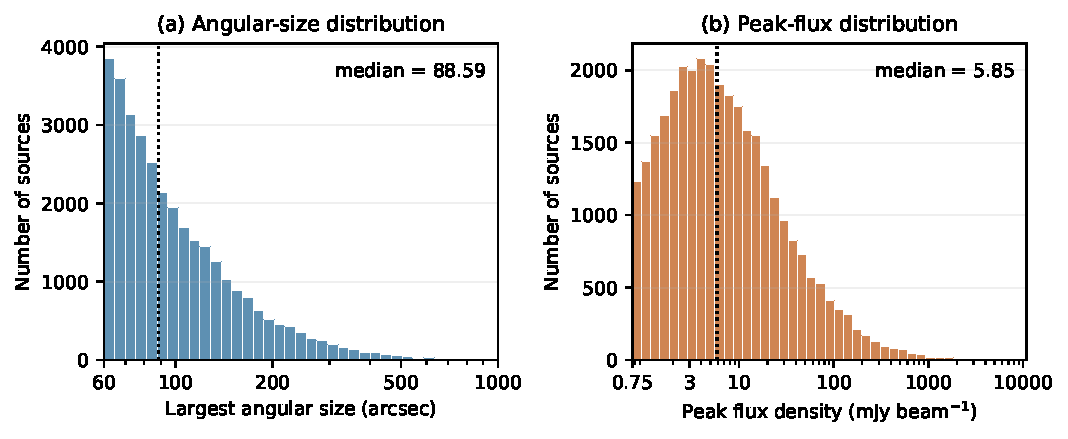
\includegraphics[width=\linewidth]{img/data_sample_distributions.pdf}
  \caption[Angular-size and peak-flux-density distributions]{Largest-angular-size and peak-flux-density distributions of the
    32\,514 sources in the processed catalogue sample. Both horizontal
    axes are logarithmic; dotted lines mark the sample medians.}
  \label{fig:data_sample_distributions}
\end{figure}

Each selected source is converted into a model input by the preprocessing pipeline of \citet{Nicolas2025}:
\begin{enumerate}
\item A square cutout of side \(1.5\times\mathrm{LAS}\) is extracted from the corresponding mosaic and centred on the host position.
\item Pixel values below \(v_{\min}=3\sigma_{\mathrm{img}}\) are set to \(v_{\min}\), where \(\sigma_{\mathrm{img}}\) is the sigma-clipped standard deviation of the cutout, estimated with a \(3\sigma\) rejection threshold and at most ten iterations. This suppresses background fluctuations and low-intensity artefacts.
\item The clipped image is then resampled to \(128\times128\) pixels using scikit-image's default first-order interpolation for floating-point arrays, min--max normalised to \([0,1]\), and stored as an 8-bit single-channel greyscale image.
\end{enumerate}
Because the cutout side scales with the LAS, sources of very different angular size appear at a comparable scale in the frame, so that the network input is dominated by morphology.

\begingroup
\emergencystretch=2em
The model receives linearly min--max-normalised intensities. For visual inspection, the representative-source galleries use a symmetric-logarithmic intensity display to reveal faint structure. Only the archived raw-cluster panels retain their original display scaling.
\par
\endgroup

\subsection{External reference catalogues}
\label{sec:data_external}

We used three independently constructed morphological catalogues (Table~\ref{tab:external_individual_samples}) of LoTSS-DR2 sources exclusively for comparison (Sec.~\ref{sec:results_external}).
\begin{table}[h]
\centering
\small
\setstretch{1}
\setlength{\tabcolsep}{4pt}
\renewcommand{\arraystretch}{1.25}
\begin{tabular*}{\linewidth}{@{}p{0.15\linewidth}@{\extracolsep{\fill}}p{0.35\linewidth}rrrr@{}}
\toprule
Catalogue & Description & \shortstack[r]{Full\\catalogue} & Matched & Mapped & \shortstack[r]{Mapped,\\curated\\excluded} \\
\midrule
\raggedright\citet{Clews2025} & \raggedright Semi-automated ridgeline analysis covering classical radio-galaxy morphologies. & 20\,172 & 11\,062 & 8\,402 & 7\,757 \\
\addlinespace
\raggedright\citet{Horton2025} & \raggedright Visual inspection with multi-attribute labels, including hybrid and precession-related signatures. & 9\,985 & 9\,287 & 9\,070 & 8\,352 \\
\addlinespace
\raggedright\citet{Chilufya2025} & \raggedright Classification of extended radio-loud AGN selected with \(\mathrm{LAS}>60''\). & 2\,828 & 2\,788 & 2\,788 & 2\,590 \\
\bottomrule
\end{tabular*}
\caption[Individual reference-catalogue selections]{Reference catalogues and source counts after identifier matching, morphology mapping and exclusion of internally curated sources.}
\label{tab:external_individual_samples}
\end{table}

Firstly, we cross-compared each catalogue with our primary dataset by matching their \texttt{Source\_Name} identifiers. These are flagged as \textbf{Matched} in Table~\ref{tab:external_individual_samples}.
We then translate the reference labels into our morphology classes using the rules in Sec.~\ref{sec:method_external_mapping}, retaining sources with usable labels as the \textbf{Mapped} sample.
Reference labels come from Clews's \texttt{Morph}, Horton's boolean flags and Chilufya's \texttt{Final\_Morph} (\nolinkurl{radio_optical_class-v1}).
In Sec.~\ref{sec:results_external}, we report \(F_1\) first for the \textbf{Mapped, curated excluded} samples, which remove overlap with supervised training, and then for the full \textbf{Mapped} samples.

Besides individual usage of these three catalogues, we used sources with identical mapped labels in all three catalogues. Table~\ref{tab:external_combined_samples} details each sample and its purpose.  

\begin{table}[H]
\centering
\small
\setstretch{1}
\setlength{\tabcolsep}{4pt}
\renewcommand{\arraystretch}{1.25}
\begin{tabular*}{\linewidth}{@{}p{0.26\linewidth}@{\extracolsep{\fill}}rp{0.60\linewidth}@{}}
\toprule
Sample & Sources & Definition \\
\midrule
At least one mapped reference & 16\,177 & Unique study sources with a usable label in at least one catalogue; used for score distributions. \\
Common-source sample & 404 & Study sources present in all three catalogues, regardless of label availability. \\
Common mapped sample & 311 & Common sources with usable mapped labels in all three catalogues. \\
Consensus sample & 149 & Common mapped sources assigned the same morphology by all three catalogues. \\
Consensus excluding curated sources & 139 & Consensus sources remaining after removing the internally curated sample. \\
\bottomrule
\end{tabular*}
\caption[Combined reference-catalogue selections]{Definitions and source counts for combined reference-catalogue selections.}
\label{tab:external_combined_samples}
\end{table}

\subsection{Radio-relic reference sample}
\label{sec:data_relics}

For the diffuse-emission application in Sec.~\ref{sec:method_relics}, we select ten radio relics from a yet-unpublished catalogue compiled by The Tautenburg Radio Relic Collection team under the supervision of Prof. Dr. Matthias Hoeft. Table~\ref{tab:relic_sample} lists their relic-centred coordinates and largest angular sizes (LAS), which we use directly to construct the cutouts from LoTSS-DR3. Their host clusters and the reference positions are also provided for identification.

\begin{table}[H]
\centering
\small
\setlength{\tabcolsep}{3pt}
\renewcommand{\arraystretch}{1.1}
\begin{tabular}{@{}lrrrlrr@{}}
\toprule
 & \multicolumn{2}{c}{Relic position} & & & \multicolumn{2}{c}{Cluster position} \\
\cmidrule(lr){2-3}\cmidrule(l){6-7}
Relic & RA & Dec & LAS & Host cluster & RA & Dec \\
\midrule
P113 N      & 4.9363 & 25.3543 & 228 & PSZ2 G113.91-37.01 & 4.9129 & 25.2908 \\
Toothbrush D & 90.9042 & 42.1708 & 66 & RX J0603.3+4214 & 90.825 & 42.2333 \\
Toothbrush B & 90.8333 & 42.3083 & 474 & RX J0603.3+4214 & 90.825 & 42.2333 \\
MS1752 SW   & 267.9745 & 44.6325 & 192 & MACS J1752.0+4440 & 268.009 & 44.6773 \\
MS1752 NE   & 268.0829 & 44.6953 & 270 & MACS J1752.0+4440 & 268.009 & 44.6773 \\
Zw2341 RS   & 355.95 & 0.23 & 216 & ZwCl 2341.1+0000 & 355.919 & 0.3053 \\
P096p N     & 284.1583 & 66.4417 & 204 & PSZ1 G096.89+24.17 & 284.16 & 66.3861 \\
P096p S     & 284.1875 & 66.3292 & 330 & PSZ1 G096.89+24.17 & 284.16 & 66.3861 \\
P116 N      & 8.0645 & 18.1766 & 103.8 & PSZ2 G116.50-44.47 & 8.0342 & 18.1069 \\
A2256 R1    & 256 & 78.7667 & 600 & Abell 2256 & 255.9064 & 78.623 \\
\bottomrule
\end{tabular}
\caption[Selected radio relics and host clusters]{Selected relics and their host clusters. Coordinates are in degrees and LAS in arcseconds.}
\label{tab:relic_sample}
\end{table}

We note that the original FITS headers give a circular \(9''\) beam for Zw2341 RS and \(6''\) beams for the other nine selected cutouts. Nevertheless, the relic inputs share the final pixel dimensions, not a uniform native angular resolution.
